%\documentclass[10pt,a4paper,twoside,twocolumn,draft]{book}
\documentclass[10pt,a4paper,twoside,twocolumn]{book}

\usepackage[utf8]{inputenc}
\usepackage[frenchb]{babel}

% polices de caractères pour les titres et le texte et formules

\usepackage[condensed]{roboto} 
\usepackage[sfdefault,bitstream-charter]{mathdesign}
\usepackage[T1]{fontenc}

% mathématiques et schémas

\usepackage{amsmath}
\usepackage{bm}
\usepackage{graphicx}
\usepackage{cancel}
%\usepackage{fourier}

% tables et tableaux

\usepackage{tabu} 
\usepackage{float} 
\usepackage{multirow}
\usepackage{footnote}

% Mise en page 

\usepackage[left=2cm,right=2cm,top=2.5cm,bottom=3cm,bindingoffset=1.5cm, footskip=1.5cm]{geometry}

% couleurs

\usepackage{color}
\usepackage[svgnames]{xcolor}
%\definecolor{couleurtitres}{rgb}{0.12,0.47,0.87}
\definecolor{couleurtitres}{gray}{0.0}
\definecolor{couleur_exercice}{rgb}{0.36, 0.54, 0.66}	
\definecolor{corriger}{rgb}{0.0, 0.5, 0.0}	

% numéros de pages en bas de page et entetes de page

\usepackage{fancyhdr}
\pagestyle{fancy}
\fancyhf{}
\fancyfoot[CE,CO]{ \mdseries \sffamily \thepage}
\renewcommand{\headrulewidth}{0pt}
\fancyhead[LO]{\color{couleurtitres} \mdseries \sffamily \leftmark}
\fancyhead[LE]{\color{couleurtitres}  \mdseries \sffamily
		    \MakeUppercase{physique chimie 2\ieme}} 
%     	nécessaire pour avoir le même style de numéro de page sur les
%	pages de chapitre
\fancypagestyle{plain}{%
\fancyhf{} % 
\fancyfoot[CE,CO]{ \mdseries \sffamily \thepage}}


% modification du format des titres

\usepackage[explicit]{titlesec}
% 						correctif du bug de titlesec qui n'affiche plus les numéros de section
\usepackage{etoolbox}
\makeatletter
\patchcmd{\ttlh@hang}{\parindent\z@}{\parindent\z@\leavevmode}{}{}
\patchcmd{\ttlh@hang}{\noindent}{}{}{}
\makeatother
% 						fin  du correctif du bug 

\titleformat{\chapter}%
		[display]% style : hang, display, runin, leftmargin, ...
		{\mdseries \sffamily }% changement de fonte numéro + titre
		{ \colorbox{gray}{ \large  \color{white} \bfseries \chaptertitlename~\thechapter}}% numéro
		{10pt}% espace entre le numéro et le titre
		{\color{couleurtitres} \Huge  #1	}% changement de fonte du titre
		
\titleformat{\section}%
		{\mdseries \sffamily \large}
		{\color{couleurtitres} \bfseries \thesection }
		{1em}
		{\color{couleurtitres} \bfseries  #1}
		[{\titlerule[1pt]}]
		
\titleformat{\subsection}
		%[hang]
		{\mdseries \sffamily}
		{\color{couleurtitres} \bfseries \thesubsection}
		{1em}
		{\color{couleurtitres} \bfseries #1 }		


% commande pour générer le paragraphe d'intro des chapitres

\newcommand{\intro}[1]{ %\noindent 
				\fcolorbox{black}{white}{%Azu
				    \begin{minipage}{6.0cm} 
						\bfseries Introduction \\
						 \mdseries \em #1  
				    \end{minipage} 
				}
		}
		

%	Figures

\usepackage{graphicx}
\graphicspath{{images/}}
\usepackage[format=plain,
            labelfont=it,
            textfont=it]{caption}	

% Formules chimiques            

\usepackage{chemfig}
\usepackage[version=3]{mhchem}
\makeatother
\setdoublesep{0.35700 em}  % 'Bond Spacing'
\setatomsep{2.0em}    % 'Fixed Length'
\setbondoffset{0.18265 em} % 'Margin Width'
\newcommand{\bondwidth}{0.06642 em} % 'Line Width'
\setbondstyle{line width = \bondwidth}
\renewcommand*{\printatom}[1]{{\sffamily\cf{#1}}}
            
%  Hyperliens

\usepackage{hyperref}
\hypersetup{
    colorlinks=true,
    linkcolor=blue,
    filecolor=blue,      
    urlcolor= blue,
}
      

% Exercices

\newcounter{numexos}		%Création d'un compteur qui s'appelle numexos
\setcounter{numexos}{0}		%initialisation du compteur
\newcommand{\exercice}[1]	{%Création d'une macro ayant un paramètre
    \addtocounter{numexos}{1}	%chaque fois que cette macro est appelée, 
				%elle ajoute 1 au compteur numexos    				
    \noindent\fbox{\thenumexos}  #1  \par  % Met en rouge Exercice et la 
					% valeur du compteur appelée 
					% par \thenumeexos
}
\newcounter{numcorrs}		%Création d'un compteur qui s'appelle numexos
\setcounter{numcorrs}{0}		%initialisation du compteur
\newcommand{\correction}[1]	{%Création d'une macro ayant un paramètre
    \addtocounter{numcorrs}{1}	%chaque fois que cette macro est appelée, 
				%elle ajoute 1 au compteur numexos
     \noindent\fbox{\thenumcorrs} #1 \par 
}      
      

% informations sur le document

\author{Wulfran Fortin}
\title{Cours de Physique Chimie  2de}

% pour les tests

\usepackage{lipsum}

\begin{document}
\pagenumbering{roman}

\begin{titlepage}
		\fontfamily{phv}\selectfont \color{couleurtitres}
		\vspace*{\stretch{1}}
		\begin{flushright} \LARGE
			Classe de seconde
		\end{flushright}
		\hrule
		\begin{flushleft}
			\Huge\mdseries
			\MakeUppercase{Physique chimie}
		\end{flushleft}
		\vspace*{\stretch{2}}
		\begin{center}
			\includegraphics[width=12cm]{images/dessinCouvertureLivre.png}
		\end{center}
		\vspace*{\stretch{2}}
		\begin{center}
			Wulfran Fortin (2019)
		\end{center}
\end{titlepage}

%%%%%%%%%%%%%%%%%%%%%%%%%%%%%%%%%%%%%%%%%%%%%%%%%%%%%%%%%%%%%%%%%%%%%

%\paragraph{Illustration de couverture}%
%Cercle de Borda. \\
%\textit{<<Exposé des opérations faites en France en 1787 pour la 
%jonction des observatoires de Paris et de Greenwich>>} \\
%Cassini Jean-Dominique, Méchain Pierre, Legendre Adrien-Marie\\
%Bibliothèque nationale de France
%\paragraph{Principe} Le cercle répétiteur était un instrument de géomètre
%pour mesurer très précisément des angles. Il s'agissait à l'époque de mesurer
%par triangulation la longueur d'une portion du méridien nord-sud traversant 
%la France. Ensuite, connaissant la longueur totale d'un quart de méridien et 
%en le divisant en $ \frac{1}{10 000 000}$ parties, on a obtenu la première 
%définition du \textit{mètre étalon} qui permit ensuite la première 
%définition du \textit{kilogramme étalon} (la masse d'un cube de $10~cm$
%d'arête contenant de l'eau pure à $4~ {}^oC$. Ce fût l'origine du 
%\textit{système internationale d'unités SI}.

\setcounter{tocdepth}{1}

\tableofcontents

\mainmatter

%%%%%%%%%%%%%%%%%%%%%%%%%%%%%%%%%%%%%%%%%%%%%%%%%%%%%%%%%%%%%%%%%%%%%
\chapter{Description et caractérisation de la matière à l'échelle macroscopique}

\intro{À notre échelle, la matière nous apparaît sous forme solide, liquide ou gazeuse.
 Elle est constituée d'une même espèce chimique ou peut être un mélange en apparence 
homogène ou hétérogène. Le chimiste ou le physicien va pouvoir analyser la composition
de la matière en pesant et mesurant des volumes de matière.}

%%%%%%%%%%%%%%%%%%%%%%%%%%%%%%%%%%%%%%%%%%%%%%%%%%%%%%%%%%%%%%%%%%%%%
\section{Corps purs et mélanges}

\subsection{Corps pur}
\paragraph{Définition} Un \textit{corps pur} est composé d'une seule espèce
chimique.
\paragraph{Exemple} L'eau distillée ne contient que des molécules d'eau
$H_2 O$, le cuivre pur ne contient que les atomes de $Cu$, le dioxygène
n'est constitué que de molécules $O_2$.

\subsection{Mélange} 
\paragraph{Définition} Un \textit{mélange contient plusieurs espèces chimiques}.
Le mélange est \textit{homogène} si les espèces chimiques ne sont
pas discernables. Dans le cas contraire, le mélange est \textit{hétérogène}.
\paragraph{Exemple} L'air, l'eau salée ou sucrée sont des mélanges homogènes.
Le sang, le lait sont des mélanges hétérogènes.


\subsection{Identification d'espèces chimiques par des méthodes physiques}
\paragraph{Méthodes physiques} Une \textit{espèce chimique} peut être identifiée 
par
\begin{itemize}
 \item ses températures de changement d'état
 \item sa masse volumique $ \rho$ par rapport à celle de l'eau 
\end{itemize}
La masse volumique de l'eau vaut $ \rho = 1.0~g.mL^{-1}$.

\paragraph{Masse volumique $\rho$} La \textit{masse volumique $\rho$} d'un corps (solide, liquide ou gaz) est le coefficient de proportionnalité entre sa masse $m$ et son volume $V$. 
$$ m = \rho \times V$$
L'unité de la masse volumique dépend des unités choisies pour la masse et le volume. Si $m$ est en gramme ($g$) et $V$ en millilitre ($mL$) alors $\rho$ est en gramme par millilitre ($g.mL^{-1}$).


\subsection{Identification d'espèces chimiques par des méthodes chimiques}
\paragraph{Test de présence de l'eau} 
La présence d'eau peut être mise en évidence par le test au sulfate de cuivre anhydre, poudre de
couleur blanche, qui devient bleue en présence d'eau. On peut verser une goutte de liquide à 
tester dessus ou déposer un peu de poudre sur un solide où on cherche la présence d'eau (figure 
\ref{fig:test_presence_eau}).
\begin{figure}[h]
  \begin{center}
      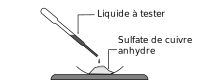
\includegraphics[width=\columnwidth]{1.1.-melanges/test_presence_eau.pdf}
  \end{center}
  \caption{La présence d'eau est confirmée par la coloration en bleu du sulfate de cuivre anhydre}
  \label{fig:test_presence_eau}
\end{figure}

\paragraph{Test de présence du dihydrogène}
Le dihydrogène $H_2$ se détecte par le test de la flamme qui provoque une petite explosion (figure 
\ref{fig:test_presence_H2}).
Attention, la quantité de gaz à tester doit être très faible, dans un petit tube à essai, 
car la réaction de combustion est très violente!
\begin{figure}[h]
  \begin{center}
      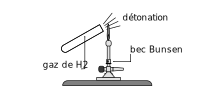
\includegraphics[width=\columnwidth]{1.1.-melanges/test_presence_H2.pdf}
  \end{center}
  \caption{La présence de dihydrogène est confirmée par une explosion. Attention, ce test doit être
  fait avec de très petites quantités de gaz, l'explosion étant très violente.}
  \label{fig:test_presence_H2}
\end{figure}

\paragraph{Test de présence du dioxygène}
Le dioxygène se détecte en plaçant un charbon incandescent dans un récipient où il y a du dioxygène.
Le charbon va s'enflammer grâce à l'oxygène (figure \ref{fig:test_presence_O2}).
\begin{figure}[h]
  \begin{center}
      \includegraphics[width=\columnwidth]{1.1.-melanges/test_presence_O2.pdf}
  \end{center}
  \caption{La présence de dioxygène ravive une flamme à l'extrémité d'un bout de bois incandescent.}
  \label{fig:test_presence_O2}
\end{figure}

\paragraph{Test de présence du dioxyde de carbone}
Le dioxyde de carbone se détecte en faisant barboter le gaz dans de l'eau de chaux, qui va se troubler à
cause de la formation d'un précipité (figure \ref{fig:test_presence_CO2}).
\begin{figure}[h]
  \begin{center}
      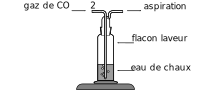
\includegraphics[width=\columnwidth]{1.1.-melanges/test_presence_CO2.pdf}
  \end{center}
  \caption{La présence de dioxyde de carbone trouble l'eau de chaux où barbote le gaz à tester.}
  \label{fig:test_presence_CO2}
\end{figure}


%%%%%%%%%%%%%%%%%%%%%%%%%%%%%%%%%%%%%%%%%%%%%%%%%%%%%%%%%%%%%%%%%%%%%
\section{Composition d'un mélange}
\subsection{Composition en masse}
\paragraph{Définition} Dans un \textit{mélange d'espèces chimiques} de masse totale $m$,
une des espèces chimiques a une masse $m_i$. On calcule alors son 
\textit{pourcentage en masse} grâce à la formule $$ \frac{m_i}{m} \times 100$$
qui s'exprime en $\%~mas $. Donner la \textit{composition en masse du mélange}
c'est donner les pourcentages en masse de tous les composants.
\paragraph{Exemples} Une solution contient $5.00~g$ d'hydroxyde de sodium $NaOH$
dans $100~g$ d'eau. La masse totale sera $m=100 + 5 = 105~g$ et donc le pourcentage
en masse d'hydroxyde sera $$\frac{5.00}{105} \times 100 = 4.77~\%~mas$$ \\
On veut savoir quelles masses de chlorure de sodium $NaCl$ et d'eau $H_{2}O$ prendre
pour avoir $175~g$ d'une solution à $15~\%~mas$ en chlorure de sodium. Si j'appelle
$a$ la masse de chlorure de sodium et $b$ la masse d'eau, je peux écrire que la masse
totale sera $$ a + b = 175~g$$ Si il y a $15~\%~mas$ en chlorure de sodium, je peux 
aussi écrire que $$ \frac{b}{175} \times 100 = 15$$ En divisant à gauche et à droite 
par $100$ puis en simplifiant $$ \frac{b}{175} = 0.15$$ et enfin en multipliant à 
gauche et à droite par $175$ et en simplifiant $$b = 26.25$$ c'est à dire qu'il faut
une masse de chlorure de sodium $b=26.25~g$ qu'on dissoudra dans une masse $a = 175 -b=
148.75~g$ d'eau.
\subsection{Composition en volume}
\paragraph{Définition}Dans un mélange d'espèces chimiques de volume total $V$, 
une des espèces chimiques a un volume $V_i$. On calcule alors son 
\textit{pourcentage en volume} grâce à la formule $$ \frac{V_i}{V} \times 100$$
qui s'exprime en $\%~vol $. Donner la \textit{composition en volume du mélange}
c'est donner les pourcentages en volume de tous les composants.
\paragraph{Cas de l'air} L'air que nous respirons a la composition en volume moyenne
suivante (tableau \ref{tab:composition_atmosphere}).
\begin{table}[h!]
  \centering
  \begin{tabu} to 0.95\linewidth {  X[2,l]  X[c]  }
    \hline
      \multirow{2}{4em}{\textbf{Élément}} & \textbf{Volume} \\
				      & \textbf{(en $\%~vol$)} \\
    \hline
      Azote $N_2$ & $78.09$ \\
      Oxygène $O_2$ & $20.95$ \\
      Argon $Ar$ & $0.93$ \\
      Dioxyde de carbone $CO_2$ & $0.035$ \\
      Autres gaz &  $...$ \\ 
    \hline
  \end{tabu}
  \caption{Composition en volume de l'atmosphère terrestre}
  \label{tab:composition_atmosphere}
\end{table}
\paragraph{Exemple} Si on prend un volume d'air $V=5.2~L$, alors
d'après le tableau \ref{tab:composition_atmosphere}, comme la 
composition en volume en azote est de $78.09~\%$, on peut écrire
$$ \frac{V_i}{5.2~L}\times 100 = 78.09$$ On divise à gauche et à droite 
par $100$ puis on multiplie à gauche et à droite par $5.2~L$, on
a alors le volume d'azote $$V_i = 4.1~L$$


%%%%%%%%%%%%%%%%%%%%%%%%%%%%%%%%%%%%%%%%%%%%%%%%%%%%%%%%%%%%%%%%%%%%%
\section{Solutions aqueuses}
\subsection{Solution}
\paragraph{Définition} Une \textit{solution} se constitue d'un liquide
\textit{le solvant} dans lequel est dissout \textit{le soluté} qui est
une espèce chimique moléculaire ou ionique. Voir la figure \ref{fig:solution}. Si le solvant est de l'eau,
on parle de \textit{solution aqueuse}.
\begin{figure}[h!]
  \begin{center}
      \includegraphics[width=0.8\columnwidth]{1.3.-schema-solution/schema_solution.pdf}
  \end{center}
  \caption{Une solution se compose d'un soluté dissout dans un solvant}
  \label{fig:solution}
\end{figure}


\subsection{Concentration en masse}
\paragraph{Définition} La \textit{concentration en masse $Cm$} d'une solution
est le rapport entre la masse $m$ de \textit{soluté} présent et le volume
$V$ de \textit{solution} $$Cm = \frac{m}{V}$$
Les unités sont
\begin{itemize}
 \item pour la masse $m$: le gramme $g$
 \item pour le volume $V$: le litre $L$
 \item pour la concentration en masse $Cm$: le gramme par litre $g.L^{-1}$
\end{itemize}

\subsection{Concentration maximale}
\paragraph{Définition} Pour un \textit{soluté donné}, il existe une 
\textit{concentration maximale} que l'on peut atteindre et au delà de laquelle
le \textit{soluté apporté} n'est plus capable de se dissoudre dans le solvant. Voir figure \ref{fig:solution_saturee}.
\begin{figure}[h!]
  \begin{center}
      \includegraphics[width=\columnwidth]{1.3.-schema-solution/solution_saturee.pdf}
  \end{center}
  \caption{Une solution de concentration en masse théorique $t$ supérieure à une concentration maximale $t_{max}$ ne sera 
  pas réalisable, car il restera du solide impossible à dissoudre car la concentration maximale est atteinte.}
  \label{fig:solution_saturee}
\end{figure}

\paragraph{Exemple}
On peut dissoudre au maximum $358~g$ de chlorure de sodium dans $1.00~L$ d'eau à $20~{}^o C$. 
Pour le chlorure d'argent, on peut dissoudre dans $1~L$ d'eau pur seulement $2,4~mg$ de ce sel.
Pour le glucose, on peut dissoudre dans un litre d'eau environ $900~g$ de cristaux de glucoses.

\subsection{Réalisation d'une solution} Pour fabriquer un volume $V$
de solution de \textit{concentration en masse} $Cm$, on doit peser une masse $m$
de soluté de manière à avoir une concentration en masse $$Cm=\frac{m}{V}$$
Ensuite, on procède à sa dissolution dans une fiole jaugée de volume $V$.
Voir figure \ref{fig:fab-sol-dissolution} page \pageref{fig:fab-sol-dissolution}.

\begin{figure*}[h!]
  \begin{center}
      \includegraphics[width=\textwidth]{1.3.-schema-solution/fab-sol-dissolution.pdf}
  \end{center}
  \caption{Fabrication d'une solution par dissolution}
  \label{fig:fab-sol-dissolution}
\end{figure*}


\subsection{Dilution d'une solution}
Si on a une \textit{solution mère} de concentration en masse $Cm_{\text{mère}}$
et de volume $V_\text{mère}$ on peut fabriquer une \textit{solution fille} de volume
$V_\text{fille}$ et de concentration $Cm_\text{fille}$ en ajoutant du solvant et on aura la relation $$ V_\text{fille} \times Cm_\text{fille} = V_\text{mère} \times Cm_\text{mère}$$
Voir figure \ref{fig:fab-sol-dilution} page \pageref{fig:fab-sol-dilution}.

\begin{figure*}[h!]
  \begin{center}
      \includegraphics[width=\textwidth]{1.3.-schema-solution/fab-sol-dilution.pdf}
  \end{center}
  \caption{Fabrication d'une solution par dilution.}
  \label{fig:fab-sol-dilution}
\end{figure*}


%%%%%%%%%%%%%%%%%%%%%%%%%%%%%%%%%%%%%%%%%%%%%%%%%%%%%%%%%%%%%%%%%%%%%
\section{Dosage par étalonnage}
\subsection{Dosage}
\paragraph{Définition}
Faire un \textit{dosage} en chimie, c'est \textit{mesurer la
concentration} d'une espèce chimique dans une solution. Pour mesurer 
cette concentration, on utilise des méthodes physiques ou chimiques.
\paragraph{Exemple} Les grandeurs que l'on peut utiliser pour mesurer
une concentration peuvent être la masse volumique, la couleur, la conductivité
électrique, le pH, etc. ...

\subsection{Étalonnage}
\paragraph{Définition}
Pour réaliser un \textit{dosage par étalonnage} d'une espèce chimique en solution, on \textit{fabrique
des solutions étalons} dont on connaît précisément la concentration et on mesure une grandeur
physique correspondant à cette solution. Ensuite, après avoir tracé une \textit{courbe 
d'étalonnage}, on mesure la même grandeur physique pour la solution inconnue et on en déduit 
la valeur de sa concentration \textit{par comparaison}.
\paragraph{Exemple}
Pour doser le saccharose dans $1~L$ de \textit{Coca Cola}, on a fabriqué par dissolution quatre solutions étalons de $100~mL$ de concentration en masse précise dont on mesure ensuite la masse volumique $\rho $. On trace   la masse volumique en fonction de la concentration en masse, puis après avoir mesuré la masse volumique du Coca Cola, on en déduit la concentration en masse en saccharose $t_{\textit{Coca Cola}} = 106~g.L^{-1}$.
Voir figure \ref{fig:courbe_etalonnage_cocacola}.
\begin{figure}[h!]
  \begin{center}
      \includegraphics[width=0.9\columnwidth]{1.3.-schema-solution/courbe_etalonnage_cocacola.pdf}
  \end{center}
  \caption{Dosage par étalonnage de la concentration en masse en saccharose du \textit{Coca Cola}.}
  \label{fig:courbe_etalonnage_cocacola}
\end{figure}

      
%%%%%%%%%%%%%%%%%%%%%%%%%%%%%%%%%%%%%%%%%%%%%%%%%%%%%%%%%%%%%%%%%%%%%

\chapter{Modélisation de la matière à l'échelle microscopique}


\intro{À l'échelle microscopique, la matière est décrite comme étant un ensemble d'atomes constitués
d'un noyau qui contient des protons et des neutrons, et qui est entouré d'un cortège électronique,
dont l'organisation en couches et sous couches permet d'expliquer les propriétés chimiques des 
éléments du tableau de la classification périodique. Ces atomes pourront s'assembler, entre autre, 
en molécules. Le chimiste développera des outils théoriques pour compter rapidement ces atomes
et ces molécules.}

%%%%%%%%%%%%%%%%%%%%%%%%%%%%%%%%%%%%%%%%%%%%%%%%%%%%%%%%%%%%%%%%%%%%%
\section{Du macroscopique au microscopique}
\subsection{Introduction}
Toute la matière à notre échelle se compose d'atomes de différentes natures
groupés en molécule et en cristaux, puis sous formes de structures de plus en plus
complexes pour aboutir aux êtres et objets de notre quotidien (figure \ref{fig:macro-vers-micro}).
\begin{figure}[!h]
  \begin{center}
      \includegraphics[width=1\columnwidth]{2.1-macro-micro/humain_vers_atome_NB.pdf}
  \end{center}
  \caption{Du macroscopique vers le microscopique}
  \label{fig:macro-vers-micro}
\end{figure}

\subsection{Entités chimiques}
\paragraph{Définition} Une \textit{entité chimique} désigne de façon
générale
\begin{itemize}
 \item un \textit{atome}
 \item une \textit{molécule} qui est un ensemble d'atomes reliés entre eux
 \item un \textit{cation}, qui est un ion positif
 \item un \textit{anion}, qui est un ion négatif
\end{itemize}
Voir figure \ref{fig:espece-vers-entite} page \pageref{fig:espece-vers-entite}.
\paragraph{Exemples}
Les \textit{atomes} de cuivre $Cu$, de fer $Fe$. Une \textit{molécule} d'eau $H_2O$, une 
\textit{molécule} d'acide éthanoïque $CH_3 COOH$, un \textit{cation} $Fe^{3+}$, 
un \textit{cation} $H_3O^{+}$, un \textit{anion} $SO_4^{2-}$, un \textit{anion}
$Cl^{-}$.

\subsection{Espèce chimique}
\paragraph{Définition} Une \textit{espèce chimique} est un ensemble d'\textit{
entités chimiques identiques}, en très grand nombre.
Voir figure \ref{fig:espece-vers-entite} page \pageref{fig:espece-vers-entite}.

\paragraph{Exemples} L'eau liquide est une espèce chimique qui contient un grand 
nombre de molécules d'eau, voir la figure \ref{fig:espece-vers-entite-glace-eau}.\\ Le sel de cuisine est une espèce chimique qui contient
un grand nombre de cations $Na^{+}$ et d'anions $Cl^{-}$, l'or est une espèce chimique
qui contient un grand nombre d'atomes d'or $Au$ (\textit{Aurum} l'or en latin).

\begin{figure}[!h]
  \begin{center}
      \includegraphics[width=1\columnwidth]{2.1-macro-micro/espece-entite-v2.pdf}
  \end{center}
  \caption{De l'espèce chimique vers l'entité chimique}
  \label{fig:espece-vers-entite}
\end{figure}

\begin{figure}[!h]
  \begin{center}
      \includegraphics[width=1\columnwidth]{2.1-macro-micro/espece-entite-glace-eau.pdf}
  \end{center}
  \caption{La glace d'eau est une espèce chimique constituée de molécules d'eau régulièrement empilées}
  \label{fig:espece-vers-entite-glace-eau}
\end{figure}

\subsection{Électro-neutralité de la matière }
\paragraph{Définition} À \textit{notre échelle}, la matière est \textit{électriquement 
neutre}, toutes les charges électriques positives se compensent avec le même nombre
de charges électriques négatives.
Les anions et les cations seront donc présents dans des proportions qui 
permettent d'assurer cette électro-neutralité.
Les atomes et les molécules ont une charge électrique nulle.
\paragraph{Exemples} La neutralité de structures ioniques comme les sels se fait
de manière à ce que les charges électriques de tous les cations neutralisent celles
de tous les anions.\\
Le \textit{chlorure de Fer III} est utilisé en faible quantité pour le traitement des
eaux usées comme \textit{floculant} qui permet de décanter plus rapidement les 
fines particules solides dans les eaux usagées. Sa formule est $FeCl_3$ et le cristal
est un assemblage régulier de cations $Fe^{3+}$ et d'anions $Cl^-$. Les \textit{trois} charges
positives de l'ion $Fe^{3+}$ sont compensées par \textit{une} charge négative 
de \textit{trois} ions $Cl^-$


%%%%%%%%%%%%%%%%%%%%%%%%%%%%%%%%%%%%%%%%%%%%%%%%%%%%%%%%%%%%%%%%%%%%%
\section{Le noyau de l'atome}

\subsection{Particules élémentaires}
\paragraph{Définition}
Les \textit{particules élémentaires} constituants les atomes sont \textit{l'électron, le proton} et 
\textit{le neutron}. Voir le tableau \ref{tab:masse-particules-elementaires} page 
\pageref{tab:masse-particules-elementaires} et le tableau \ref{tab:charge-particules-elementaires} 
page \pageref{tab:charge-particules-elementaires}.

\begin{table}[!h]
  \centering
  \begin{tabu} to 0.95\columnwidth { X[l] X[l] }
      \hline 
      \textbf{Particule} & \textbf{Masse  (en $\bm{kg} $)} \\ 
      \hline \\[-10pt]
	électron & $9.11 \times 10^{-31}$ \\ 
	neutron  & $1.67 \times 10^{-27}$ \\ 
	proton   & $1.67 \times 10^{-27}$ \\ 
      \hline      
  \end{tabu}
  \caption{Masse des particules élémentaires constituant l'atome}
  \label{tab:masse-particules-elementaires}
\end{table}

\begin{table}[!h]
  \centering
  \begin{tabu} to 0.95\columnwidth { X[l] X[2,l] }
      \hline 
      \textbf{Particule} & \textbf{Charge électrique   (en $\bm{C} $)} \\
      \hline \\[-10pt]
	électron & $-1.6 \times 10^{-19}$ (on note $-1$)\\ 
	neutron  & $0$ \\ 
	proton   & $1.6 \times 10^{-19}$ (on note $+1$)\\ 
      \hline      
  \end{tabu}
  \caption{Charges électriques des particules élémentaires constituant l'atome}
  \label{tab:charge-particules-elementaires}
\end{table}

\subsection{L'atome}
\paragraph{Définition}
\begin{itemize}
  \item L'\textit{atome} se compose d'un \textit{noyau} constitué de \textit{neutrons} et de \textit{protons}, 
  autour du quel orbitent des \textit{électrons} qui forment le \textit{nuage électronique}
  (figure \ref{fig:atome}).  
  \item Un \textit{atome} est \textit{neutre}, il y a \textit{autant de charges positives} (les protons) que 
  de \textit{charges négatives} (les électrons).
  \item la \textit{taille d'un atome} est de l'ordre de $0.1~nm$. Son \textit{noyau} est $100~000$ fois plus petit,
soit $1~fm$.
\end{itemize}
\begin{figure}[!h]
    \begin{center}
	\includegraphics[width=0.8\columnwidth]{2.1-macro-micro/structure_atome_NB.pdf}
    \end{center}
    \caption{Structure simplifiée de l'atome}
    \label{fig:atome}
  \end{figure}


\subsection{Écriture conventionnelle du noyau}
\paragraph{Définition}
\begin{itemize} 
  \item  On appelle \textit{numéro atomique $Z$} le nombre de \textit{protons}
  présents dans le noyau d'un atome ou d'un ion monoatomique.
  \item On appelle \textit{nombre de masse atomique $A$} le nombre de \textit{protons 
  et de neutrons} présents dans le noyau d'un atome ou d'un ion monoatomique.
  \item Le \textit{symbole chimique} d'un élément est une lettre majuscule, parfois 
  suivie d'une minuscule permettant de le désigner. Par exemple $C$ représente l'élément carbone dont $Z=6$,
  $Na$ représente l'élément sodium où $Z=11$. 
  \item \textit{L'écriture conventionnelle} d'un noyau permet d'indiquer
  son symbole $X$, son numéro atomique $Z$ et son nombre de masse $A$. $$ ^A_Z X $$
\end{itemize}


\paragraph{Exemples} $ ^{14}_{6} C $ est un atome de carbone $C$ qui possède $Z=6$ protons et donc $N=A-Z=14-6=8$ neutrons.


\subsection{Élément chimique}
\paragraph{Définition} Un \textit{élément chimique} est totalement défini par son nombre de protons $Z$ 
dans son noyau qui lui donne son nom et son symbole $X$.
\paragraph{Exemples}$ ^{45}_{20} Ca^{2+} $ est le cation calcium, il possède $Z=20$ protons 
et $45-20=25$ neutrons. Comme il a une charge positive $2+$, cela signifie que l'atome de calcium 
a perdu $2$ électrons pour devenir le cation $Ca^{2+}$.

%%%%%%%%%%%%%%%%%%%%%%%%%%%%%%%%%%%%%%%%%%%%%%%%%%%%%%%%%%%%%%%%%%%%%
\section{Le cortège électronique de l'atome}
\paragraph{Introduction} De nombreuses expériences de spectroscopie du début du XX\ieme{} siècle
ont montré que les électrons des atomes semblent être rangés autour du noyau par couches successives.

\paragraph{Définition} 
\begin{itemize}
 \item Les électrons du cortège électronique d'un atome sont répartis dans des
    \textit{couches} numérotées à partir de $1$, et qui contiennent des \textit{sous couches}
    désignées par des lettres \textit{s} et  \textit{p}.
 \item une \textit{sous couche s} contient au maximum $2$ électrons
 \item une \textit{sous couche p} contient au maximum $6$ électrons
 \item Le remplissage des couches et sous couches se fait par énergie croissante.  
\end{itemize}
Voir la figure \ref{fig:config_electronique} page \pageref{fig:config_electronique}.
\begin{figure}[!h]
    \begin{center}
	\includegraphics[width=\columnwidth]{2.1-macro-micro/niveaux_energie_atome.pdf}
    \end{center}
    \caption{Configuration électronique des $13$ électrons de l'atome 
    d'aluminium dans son état fondamental}
    \label{fig:config_electronique}
\end{figure}

\paragraph{Exemples} L'atome d'hydrogène ne possède qu'un seul électron. La
\textit{configuration électronique} de l'atome d'hydrogène sera $1s^{1}$.\\
L'atome de carbone possède $6$ électrons. La \textit{configuration électronique} 
de l'atome de carbone sera $1s^2 2s^2 2p^2$, et il a $4$ électrons de valence sur la
couche $2$ composée des sous couches $2s$ et $2p$.\\

\paragraph{Définition} Les \textit{électrons de valence} sont les électrons de la
\textit{dernière couche remplie}. Ces électrons vont donner des propriétés 
chimiques spécifiques à un élément chimique.

\paragraph{Exemples} L'atome d'aluminium a pour structure électronique $1s^2 2s^2 2p^6 3s^2 3p^1$,
sa dernière couche remplie est la troisième couche et il a $3$ électrons de valence, dont $2$ sur 
la sous couche $3s$ et $1$ sur la sous couche $3p$.


%%%%%%%%%%%%%%%%%%%%%%%%%%%%%%%%%%%%%%%%%%%%%%%%%%%%%%%%%%%%%%%%%%%%%
\section{Vers des entités plus stables}

\subsection{Classification périodique des éléments}

\paragraph{Définition} Les éléments de \textit{la classification périodique} se regroupent
en blocs $s$ et $p$ en fonction du nombre de couches remplies. Pour chaque colonne de 
la \textit{classification périodique}, les éléments ont le même nombre d'électrons sur leur
couche de valence. Voir la figure \ref{fig:bloc_s_p} page \pageref{fig:bloc_s_p}.
\begin{figure}[!h]
    \begin{center}
	\includegraphics[width=\columnwidth]{2.1-macro-micro/classification_blocs.pdf}
    \end{center}
    \caption{Les blocs $s$ et $p$ dans la classification périodique des éléments pour
    les trois premières lignes}
    \label{fig:bloc_s_p}
\end{figure}

\paragraph{Définition} Les éléments \textit{d'une même colonne} du tableau de la classification
périodique des éléments ont le \textit{même nombre d'électrons de valence}, ce qui leur octroie 
les \textit{mêmes propriétés chimiques}: ils forme une \textit{familles chimiques d'éléments}. Chaque colonne 
correspond ainsi à une famille. Voir figure \ref{fig:classification}.
\begin{figure*}[!h]
    \begin{center}
	\includegraphics[width=\textwidth]{2.1-macro-micro/classification.pdf}
    \end{center}
    \caption{Les trois premières lignes de la classification périodique. Chaque ligne correspond au remplissage d'une couche électronique, les éléments d'une colonne ont le même nombre d'électrons de valence, les électrons de la dernière couche remplie.}
    \label{fig:classification}
\end{figure*}


\subsection{Gaz nobles}
\paragraph{Définition} La \textit{famille des gaz nobles} correspond à la \textit{dernière colonne du tableau de la
classification périodique}. Ces éléments ne forment pas de molécules ou d'ions, ils existent simplement
sous forme monoatomique: ils sont dit \textit{chimiquement stables}, on ne peut pas faire de réactions chimiques.\\
On remarque que \textit{leur dernière couche électronique} est \textit{saturée à $8$ électrons}.
\paragraph{Exemples} Configuration électronique des gaz nobles des trois premières lignes du tableau de la
classification périodique des éléments (voir table \ref{tab:config_elec_gaz_nobles}).

\begin{table}[!h]
  \centering
  \begin{tabu} to 0.95\columnwidth { X[l] X[2,l] }
      \hline 
      \textbf{Gaz noble} & \textbf{Configuration électronique} \\
      \hline \\[-10pt]
	Hélium & $1s^2$\\
	Néon & $1s^2 2s^2 2p^{6}$\\
	Argon & $1s^2 2s^2 2p^{6} 3s^2 3p^{6}$\\
      \hline      
  \end{tabu}
  \caption{Configuration électronique des gaz nobles. On observe sur la dernière couche remplie
  qu'il y a $8$ électrons: $2$ sur la sous couche $s$ et $6$ sur la sous couche $p$.}
  \label{tab:config_elec_gaz_nobles}
\end{table}

\subsection{Ions monoatomiques}
\paragraph{Définition} Les éléments du tableau de la classification périodique vont
\textit{augmenter leur stabilité chimique} en gagnant ou perdant des électrons pour\textit{ avoir
la configuration électronique} du gaz noble le plus proche dans la classification. Voir le tableau 
\ref{tab:ions_mono_atomiques} page \pageref{tab:ions_mono_atomiques}.

\begin{table*}[!h]
  \centering
  \begin{tabu} to 1.00\textwidth { X[1.3,l] X[1.6,l] X[0.8,l] X[1.8,l] X[1.3,l] }
      \hline 
      \textbf{Atome} & \textbf{Configuration électronique}  & \textbf{Gaz noble proche} &\textbf{Ion} & \textbf{Configuration électronique} \\
      \hline \\[-10pt]
	Hydrogène  $\textit{H}$		& $1s^1$ 				& $\textit{He}$ & Hydronium  $\textit{H}^+$ 		& pas d'électron 		\\
	Sodium  $\textit{Na}$ 		& $1s^2 2s^2 2p^{6} 3s^1 $  		& $\textit{Ne}$ & Ion sodium  $\textit{Na}^+$ 		& $1s^2 2s^2 2p^{6}$ 		\\
	Potassium  $\textit{K}$ 	& $1s^2 2s^2 2p^{6} 3s^2 3p^6 4s^1 $ 	& $\textit{Ar}$ & Ion potassium $\textit{K}^+$ 		& $1s^2 2s^2 2p^{6} 3s^2 3p^{6}$ \\
	Calcium  $\textit{Ca}$ 		& $1s^2 2s^2 2p^{6} 3s^2 3p^6 4s^2 $  	& $\textit{Ar}$ & Ion calcium $\textit{Ca}^{2+}$ 	& $1s^2 2s^2 2p^{6} 3s^2 3p^{6}$ \\
	Magnésium  $\textit{Mg}$ 	& $1s^2 2s^2 2p^{6} 3s^2 $  		& $\textit{Ne}$ & Ion magnésium $\textit{Mg}^{2+}$ 	& $1s^2 2s^2 2p^{6}$ 		\\
	Chlore  $\textit{Cl}$ 		& $1s^2 2s^2 2p^{6} 3s^2 3p^5$  	& $\textit{Ar}$ & Ion chlorure $\textit{Cl}^{-}$ 	& $1s^2 2s^2 2p^{6} 3s^2 3p^6$ 	\\
	Fluor  $\textit{F}$ 		& $1s^2 2s^2 2p^{5}$  			& $\textit{Ne}$ & Ion fluorure $\textit{F}^{-}$ 	& $1s^2 2s^2 2p^{6}$ 		\\
      \hline      
  \end{tabu}
  \caption{Les cations se forment en perdant des électrons pour avoir la même configuration électronique qu'un gaz noble. Les
  anions se forment en capturant des électrons pour avoir la configuration électronique d'un gaz noble }
  \label{tab:ions_mono_atomiques}
\end{table*}
\paragraph{Exemple} L'atome de sodium $Na$ a pour structure électronique $1s^2 2s^2 2p^{6} 3s^1 $. Le gaz noble le plus
proche dans la classification périodique est le néon de structure électronique $1s^2 2s^2 2p^{6}$. Le sodium va donc \textit{perdre 
un électron} pour avoir la même configuration électronique que le gaz noble. On forme alors l'ion $Na^+$ qui a comme 
configuration électronique $1s^2 2s^2 2p^{6}$.\\
L'atome de chlore $Cl$ a pour configuration $1s^2 2s^2 2p^{6} 3s^2 3p^5$ et il lui manque seulement un électron pour avoir celles de l'Argon.
Il va donc facilement capturer un électron ailleurs pour former l'ion chlorure $Cl^-$ de configuration électronique $1s^2 2s^2 2p^{6} 3s^2 3p^6$.\\
À noter que la mise en présence de sodium métallique (atomes de $Na$) et de gaz de dichlore ($Cl_2$) produit une très vive réaction, le chlore arrachant
un électron au sodium.

\subsection{Molécules}
\paragraph{Définition} Une \textit{molécule} est un ensemble d'atomes reliés entre eux par des \textit{liaisons chimiques}
qui sont un \textit{partage d'une ou plusieurs paires d'électrons} afin que chaque atome puisse s'entourer de \textit{$8$ électrons}
pour avoir la même configuration électronique qu'un gaz noble. Voir figure \ref{fig:liaison-covalente}.
\begin{figure}[!h]
  \begin{center}
      \includegraphics[width=1\columnwidth]{2.1-macro-micro/liaison_covalente.pdf}
  \end{center}
  \caption{Partage de deux électrons entre deux atomes pour former une liaison covalente.}
  \label{fig:liaison-covalente}
\end{figure}
\paragraph{Définition} En 1916, le physico-chimiste américain Gilbert Newton Lewis propose un modèle simplifié pour expliquer la formation des molécules par le
partage de paires d'électrons. Tout atome d'une molécule sera entouré par \textit{$4$ paires d'électrons} lui permettant d'avoir sa couche de valence 
saturée à $8$ électrons comme un gaz noble. L'atome d'hydrogène n'aura qu'une seule paire d'électrons dans une molécule.\\ 
Les paires d'électrons servant à faire une liaison seront des \textit{doublets liants}, les paires d'électrons non engagées
dans une liaison seront des \textit{doublets non liants}. Voir figure \ref{fig:exemple_hcn}.
\begin{figure}[!h]
  \begin{center}
      \includegraphics[width=1\columnwidth]{2.1-macro-micro/exemple_HCN.pdf}
  \end{center}
  \caption{Formation de liaisons covalentes dans l'acide cyanhydrique. Chaque atome s'entoure de huit électrons en formant une ou plusieurs liaisons covalentes. }
  \label{fig:exemple_hcn}
\end{figure}
\paragraph{Exemples} Dans les schémas suivants, tous les atomes sont entourés par $4$ doublets, liants ou non liants, seuls les atomes
d'hydrogènes sont entourés d'un seul doublet.
\begin{itemize}
 \item l'eau  \chemfig{ H- \Lewis{26,O} -H}
 \item le dioxyde de carbone \chemfig{ \Lewis{35,O}=C=\Lewis{17,O} }
 \item l'ammoniac \chemfig{ \Lewis{4,N}(-[6]H)(-[0]H)(-[2]H)}
 \item le méthane \chemfig{H-C(-[2]H)(-[6]H)-H}
 \item l'éthanol \chemfig{H-C(-[2]H)(-[6]H)-C(-[2]H)(-[6]H)-\Lewis{26,O}-H}
 \item l'éthylène \chemfig{C(-[3]H)(-[5]H)=C(-[1]H)(-[7]H)}
 \item l'acide acétique \chemfig{H-C(-[2]H)(-[6]H)-C(=[7]\Lewis{06,O})(-[1]\Lewis{37,O}-H)}
 \item le dichlore \chemfig{\Lewis{246,Cl}-\Lewis{026,Cl}}
 \item le dihydrogène \chemfig{H-H}
 \item le dioxygène \chemfig{\Lewis{35,O}=\Lewis{17,O}}
 \item l'acide chlorhydrique \chemfig{\Lewis{246,Cl}-H}
\end{itemize}



\subsection{Énergies de liaison}
\paragraph{Définition} L'énergie de liaison est l'énergie nécessaire pour briser cette liaison. Lors d'une réaction chimique, des liaisons se brisent et 
se reforment pour obtenir de nouvelles molécules à partir des atomes présents au début.

%%%%%%%%%%%%%%%%%%%%%%%%%%%%%%%%%%%%%%%%%%%%%%%%%%%%%%%%%%%%%%%%%%%%%
\section{Compter les entités dans un échantillon de matière}
\subsection{Masse d'une entité chimique} 
\paragraph{Définition} La masse $m_e$ d'une molécule ou d'un ion polyatomique est la somme des masses des atomes qui constituent cette entité. On doit donc connaître la formule brute de l'entité.\\ La masse des atomes des trois premières lignes de la classification périodique des éléments est donnée dans le tableau \ref{tab:masse-atomes-tab-periodique}.

\paragraph{Exemple} La molécule d'eau a pour formule brute $H_2O$. Elle se compose de deux atomes d'hydrogène et d'un atome d'oxygène. Sachant que la masse d'un atome d'hydrogène est $m_H =  1.674 \times 10^{-24}~g$ et celle d'un atome d'oxygène est 
$m_O =  2.657 \times 10^{-23}~g$, on peut calculer la masse de la molécule d'eaux
\begin{equation*}
    \begin{aligned}
      m_{H_2O} =&  2 \times m_H + 1 \times m_O \\
		=& 2 \times 1.674 \times 10^{-24}~g \\
		&+ 1 \times 2.657 \times 10^{-23}~g \\
		 =& 2.992 \times 10^{-23}~g     
    \end{aligned}
\end{equation*}

\paragraph{Exemple} La molécule d'éthanol a pour formule brute $CH_3CH_2OH$. Les masses des différents atomes sont $m_H =  1.674 \times 10^{-24}~g$, $m_O =  2.657 \times 10^{-23}~g$ et $m_C =  1.995 \times 10^{-23}~g$. La masse d'une molécule d'éthanol sera alors 
\begin{equation*}
    \begin{aligned}
      m_{CH_3CH_2OH} 	=&  6 \times m_H + 1 \times m_O + 2 \times m_C\\
			=& 6 \times 1.674 \times 10^{-24}~g \\ 
			&+ 1 \times 2.657 \times 10^{-23}~g  \\
			&+ 2 \times  1.995 \times 10^{-23}~g\\
			 =& 7.651 \times 10^{-23}~g     
    \end{aligned}
\end{equation*}

\subsection{Nombre d'entités dans un échantillon}
\paragraph{Définition} Si on a un échantillon composé d'un nombre $N$ d'entités identiques ayant une masse individuelle $m_e$, alors la masse totale $m$ de l'échantillon sera le produit du nombre d'entités par la masse d'une entité
$$ m = N \times m_e$$

\paragraph{Définition} Si on connaît la masse $m$ de l'échantillon et la masse individuelle des entités $m_e$, alors on peut calculer à partir de l'équation précédente le nombre $N$ d'entités composant notre échantillon en isolant ce paramètre
\begin{equation*}
    \begin{aligned}
	  m &= N \times m_e \\
	  \frac{m}{m_e} &= \frac{N \times m_e}{m_e} \\
	  \frac{m}{m_e} &= \frac{N \times \bcancel{m_e}}{\bcancel{m_e}} \\
	  \frac{m}{m_e} &= N  
    \end{aligned}
\end{equation*}

\paragraph{Exemple} Un morceau de tube de cuivre a une masse $m$ de $1.5~kg$. Un atome de cuivre a une masse de $m_{Cu} =  1.055 \times 10^{-22}~g$. On va déterminer le nombre d'atomes de cuivre présents dans ce tube.\\ On utilise donc la formule $N= \frac{m}{m_{Cu}}$ en faisant attention aux unités:  $$m =  1.5~kg =  1500~g$$
donc le nombre d'atomes de cuivre est  $$N = \frac{1500~g}{1.055 \times 10^{-22}} = 1.42 \times 10^{25}$$
On constate que ce nombre est énorme 
$$ N = 14~500~000~000~000~000~000~000~000$$

\subsection{La mole}
\paragraph{Définition} Pour compter plus rapidement les entités présentes dans un échantillon, on les compte par paquet contenant $N_A = 6.022\times 10^{23}$ entités. Ce paquet est appelé \textit{une mole}.

\paragraph{Exemple} Si j'ai $5~mol$ d'une espèce chimique, alors mon échantillon contient un nombre totale d'entités valant $N = 5 \times N_A =  3.011\times 10^{24}$.

\paragraph{Exemple} Nous allons estimer le volume occupé par \textit{une mole} de popcorn, en supposant qu'un grain occupe le volume d'un cube de $2~cm$
d'arête. On convertit les distances en $km$ puis on calcule de volume du cube en $km^3$
$$ V_{grain} = \left( 2.00~cm \right)^3 = \left( 2.00 \times 10^{-5}~km \right)^3$$
$$ V_{grain} = 8.00 \times 10^{-15}~km^3$$
On calcule le volume occupé par la mole de popcorn 
$$ V = V_{grain} \times 6.022 \times 10^{23} = 4.8 \times 10^9 ~km^3$$
La superficie de la France est de $S=643801~km^2$, il faudrait une hauteur $h$ de pop-corn pour avoir
le volume $$V =  h \times S$$
et donc $$ h = \frac{4.80 \times 10^9~km^3}{643801~km^2} = 7500~km$$
Voir figure \ref{fig:pop_corn} page \pageref{fig:pop_corn}.
\begin{figure}[!h]
    \begin{center}
	\includegraphics[width=\columnwidth]{2.1-macro-micro/mole-pop-corn.pdf}
    \end{center}
    \caption{Une mole de popcorn couvrirait la France sur $7500~km$ de haut}
    \label{fig:pop_corn}
\end{figure}

\subsection{Quantité de matière}
\paragraph{Définition} La \textit{quantité de matière $n$} contenue dans un échantillon est le <<nombre de paquets>> contenant $6.022\times 10^{23}$ entités présent dans l'échantillon. Cette \textit{quantité de matière $n$} s'exprime en $mol$.\\
Pour calculer $n$, il faut connaître le nombre total $N$ d'entités de l'échantillon et on peut alors calculer $n$
$$n = \frac{N}{N_A}$$

\paragraph{Définition} Pour mesurer expérimentalement la quantité de matière $n$ présente dans un échantillon, il faut connaître
\begin{itemize}
 \item la formule brute de l'entité chimique constituant l'espèce chimique
 \item la masse $m$ de notre échantillon.
\end{itemize}
Ensuite, on applique les étapes de calculs de l'algorithme (voir figure \ref{fig:mesure-qte-matiere}).
\begin{figure}[!h]
    \begin{center}
	\includegraphics[width=\columnwidth]{2.1-macro-micro/mesure-qte-matiere.pdf}
    \end{center}
    \caption{Étapes du calcul d'une quantité de matière $n$ connaîssant la masse $m$ de l'échantillon et la formule brute des entités}
    \label{fig:mesure-qte-matiere}
\end{figure}

\begin{table*}[!h]
  \centering
  \begin{tabu} to 1.2\columnwidth { X[0.1,c] X[0.2,c] X[0.2,l] X[0.3,l]}
      \hline 
      \textbf{Z} & \textbf{Symbole} & \textbf{Nom} & \textbf{Masse (en $g$)} \\			
      \hline \\[-10pt]
      $1$	&H	& hydrogène	&$1.674 \times 10^{-24}$ \\
      $2$	&He	&hélium	& 	$6.647 \times 10^{-24}$ \\
      $3$	&Li	&lithium & 	$1,152 \times 10^{-23}$ \\
      $4$	&Be	&béryllium & 	$1,497 \times 10^{-23}$ \\
      $5$	&B	&bore & 	$1,795 \times 10^{-23}$ \\
      $6$	&C	&carbone &	$1,995 \times 10^{-23}$ \\
      $7$	&N	&azote & 	$2,326 \times 10^{-23}$ \\
      $8$	&O	&oxygène & 	$2,657 \times 10^{-23}$ \\
      $9$	&F	&fluor	& 	$3,155 \times 10^{-23}$ \\
      $10$	&Ne	&néon	& 	$3,351 \times 10^{-23}$ \\
      $11$	&Na	&sodium	& 	$3,818 \times 10^{-23}$ \\
      $12$	&Mg	&magnésium& 	$4,036 \times 10^{-23}$ \\
      $13$	&Al	&aluminium&	$4,481 \times 10^{-23}$ \\
      $14$	&Si	&silicium& 	$4,664 \times 10^{-23}$ \\
      $15$	&P	&phosphore& 	$5,143 \times 10^{-23}$ \\
      $16$	&S	&souffre& 	$5,324 \times 10^{-23}$ \\
      $17$	&Cl	&chlore	& 	$5,887 \times 10^{-23}$ \\
      $18$	&Ar	&argon	& 	$6,634 \times 10^{-23}$ \\
      \hline 
  \end{tabu}
  \caption{Masse des atomes des trois premières lignes du tableau de la classification périodique}
  \label{tab:masse-atomes-tab-periodique}
\end{table*}




%%%%%%%%%%%%%%%%%%%%%%%%%%%%%%%%%%%%%%%%%%%%%%%%%%%%%%%%%%%%%%%%%%%%%

\chapter{Modélisation des transformations de la matière et transfert
d'énergie}
\intro{ La matière peut se transformer en libérant ou absorbant de l'énergie.\\
Une transformation physique n'est qu'un changement de phase, solide, liquide ou gazeux, durant lequel
les molécules de la matière restent intactes. \\ Une transformation chimique transforme les molécules en
modifiant la répartition des atomes entre diverses molécules.\\ Une transformation nucléaire modifie
le noyau même de l'atome.}
%%%%%%%%%%%%%%%%%%%%%%%%%%%%%%%%%%%%%%%%%%%%%%%%%%%%%%%%%%%%%%%%%%%%%
\section{Transformation physique}
\subsection{Changement d'état}
\paragraph{Définition}Un corps pur peut être dans trois états physiques en fonction
de sa température et de la pression
\begin{itemize}
 \item solide
 \item liquide
 \item gazeux
\end{itemize}
Le passage d'un état à l'autre se fait à des températures précises selon le corps
étudié, appelées températures de changement de phase.

\paragraph{Exemples}
L'eau peut être sous forme liquide, solide (glace, neige, givre) ou à l'état 
de vapeur (voir figure \ref{fig:eau_changement_etat}).
\begin{figure}[!h]
  \begin{center}
      \includegraphics[width=1\columnwidth]{3.1-transfo-physiques/palier-fusion-eau.pdf}
  \end{center}
  \caption{Les changements d'états de l'eau à pression atmosphérique}
  \label{fig:eau_changement_etat}
\end{figure}

\paragraph{Définition} Le passage d'une phase à l'autre porte un nom spécifique, 
selon la phase de départ et celle d'arrivée ( voir figure \ref{fig:nom_changements_etats}).
\begin{figure}[!h]
  \begin{center}
      \includegraphics[width=1\columnwidth]{3.1-transfo-physiques/changements-phases.pdf}
  \end{center}
  \caption{Noms des différents types de changements d'états}
  \label{fig:nom_changements_etats}
\end{figure}

\paragraph{Remarque} La vaporisation est une évaporation avec ébullition du corps.

\subsection{Modélisation microscopique}
\paragraph{Définition} On peut modéliser les trois phases de la matière de la façon suivante
\begin{itemize}
  \item  Dans un \textit{corps pur solide}, les atomes, ions ou  molécules qui le constituent sont 
  organisés dans une \textit{structure cristalline} qui est \textit{très ordonnée et régulière}.
 
  \item Dans un \textit{corps pur liquide}, les atomes, ions ou  molécules qui le constituent 
  sont dans une \textit{structure désorganisée}, ils peuvent \textit{se déplacer}
  les uns par rapport aux autres, \textit{en restant très proches}.

  \item Dans un \textit{corps pur gazeux}, les atomes, ions ou  molécules qui le constituent 
  sont dans une \textit{structure désorganisée}, ils se déplacent à des \textit{vitesses
  importantes} et sont \textit{éloignés les uns des autres}.
\end{itemize}

\paragraph{Définition} Pour un changement d'état, lors du passage 
$solide \rightarrow liquide \rightarrow gaz$, la structure de la matière 
est de plus en plus \textit{désordonnée}.\\
Le passage $gaz \rightarrow liquide\rightarrow solide$ se caractérise par un état de plus en plus 
\textit{ordonné} de la matière.

Voir figure \ref{fig:changements-phases-structure}.

\begin{figure}[!h]
  \begin{center}
      \includegraphics[width=\columnwidth]{3.1-transfo-physiques/changements-phases-structure.pdf}
  \end{center}
  \caption{Structure de la matière dans les phases solide, liquide et gaz}
  \label{fig:changements-phases-structure}
\end{figure}

\subsection{Transfert thermique}
\paragraph{Définition} Une transformation \textit{endothermique} \textit{absorbe de l'énergie} $E$ quand elle se produit.\\
$$\textit{corps}_{\textit{solide}} + E \xrightarrow{\textit{fusion}} \textit{corps}_{\textit{liquide}}$$
$$\textit{corps}_{\textit{liquide}} + E \xrightarrow{\textit{vaporisation}} \textit{corps}_{\textit{gaz}}$$
$$\textit{corps}_{\textit{solide}} + E \xrightarrow{\textit{sublimation}} \textit{corps}_{\textit{gaz}}$$  
Une transformation \textit{exothermique} \textit{libère de l'énergie} $E$ quand elle se produit.\\
$$\textit{corps}_{\textit{liquide}} \xrightarrow{\textit{solidification}} \textit{corps}_{\textit{solide}} + E$$
$$\textit{corps}_{\textit{gaz}}  \xrightarrow{\textit{liquéfaction}} \textit{corps}_{\textit{liquide}} + E$$
$$\textit{corps}_{\textit{gaz}}  \xrightarrow{\textit{condensation~solide}} \textit{corps}_{\textit{solide}} + E$$


\paragraph{Définition} L'\textit{énergie de fusion} $E_f$ (en $J$) est l'énergie nécessaire pour faire \textit{fondre une masse} $m$ (en $kg$) d'un corps pur d'énergie massique de fusion $L_f$ (en $J.kg^{-1}$). $$ E_f = m \times L_f $$ Quand le corps se solidifie, il va libérer la même énergie. \\

L'\textit{énergie de vaporisation} $E_v$ (en $J$) est l'énergie nécessaire pour  \textit{vaporiser une masse} $m$ (en $kg$) d'un corps pur d'énergie massique de vaporisation $L_v$ (en $J.kg^{-1}$).$$ E_v = m \times L_v $$ 
Quand le corps se liquéfie, il va libérer la même énergie.


\subsection{Applications des changements d'états}
\begin{itemize}
 \item Quand on utilise une glacière, on y place des blocs de glace qui absorbent l'énergie thermique entrant dans la glacière. Tant que la glace se transforme en eau,cette énergie ne peut pas augmenter la température des objets dans la glacière.
 \item Les petites chaufferettes qui se déclenchent par un choc et où l'on observe un liquide devenant solide utilisent une espèce chimique en surfusion, et quand elle change de phase, elle libère l'énergie sous forme thermique. 
 \item Certains mammifères transpirent, l'eau en s'évaporant absorbe l'énergie thermique du corps et permet de le refroidir. 
 \item Dans les années $1970$ les sondes russes VENERA qui atterrissaient à la surface de Vénus où la température est de $400~{}^oC$, utilisaient la sublimation de nitrate de lithium tri hydraté pour absorber l'énergie thermique qui entrait dans la sonde.
 \item Les sondes spatiales utilisent un bouclier thermique pour entrer dans une atmosphère, le bouclier se sublime, ce qui permet d'évacuer une partie de l'énergie thermique due au frottement avec l'atmosphère, la sonde perd ainsi de l'énergie cinétique et est ralentie, passant à une vitesse de quelques kilomètres par seconde à quelques centaines de mètre par seconde. 
\end{itemize}

%%%%%%%%%%%%%%%%%%%%%%%%%%%%%%%%%%%%%%%%%%%%%%%%%%%%%%%%%%%%%%%%%%%%%
\section{Transformation chimique}
\subsection{Réaction chimique}
\paragraph{Définition} Lors d'une \textit{réaction chimique}, les \textit{réactifs disparaissent} pour former \textit{les produits qui apparaissent}. Il
y a \textit{conservation de la matière}, la masse reste constante, et \textit{conservation de la charge électrique}, elle reste constante lors de la réaction.

$$\textit{réactifs}  \xrightarrow{} \textit{produits} $$
$$\textit{masse des réactifs}  = \textit{masse des produits} $$
\begin{equation*}
  \begin{aligned}    
    \textit{somme des charges électriques des réactifs} &= \\
    \textit{somme des charges électriques des produits} &    
 \end{aligned} 
\end{equation*}

\subsection{Équation de réaction chimique}
\paragraph{Définition}
Une \textit{équation de réaction chimique} indique comment les atomes se réorganisent quand des réactifs réagissent pour former des produits. Cette 
équation respecte la conservation de la masse: \textit{tous les atomes présents dans les réactifs se retrouvent dans les produits} et la conservation 
de la charge électrique: \textit{la charge électrique totale de tous les réactifs est identique à la charge totale de tous les produits}.
Une équation de réaction chimique est équilibrée, les coefficients stoechiométriques indiquent en quelles proportions les réactifs réagissent entre eux
et les produits apparaissent.
\paragraph{Exemples à connaître}
\begin{itemize}
 \item combustion du carbone $$ C + O_2 \xrightarrow{} CO_2$$
 \item combustion du méthane $$ CH_4 + 2 \times  O_2 \xrightarrow{} CO_2 + 2 \times H_2O $$
 \item corrosion d'un métal par un acide $$ Zn + 2 \times H_3O^+ \xrightarrow{} Zn^{2+} + H_2 + 2 \times H_2O $$
 \item action d'un acide sur le calcaire $$ 2 \times HCl + CaCO_3  \xrightarrow{} CaCl_2 + CO_2 + H_2O $$
 \item action de l'acide chlorhydrique sur l'hydroxyde de sodium $$ H_3O^+ + Cl^- + Na^+ + OH^-  \xrightarrow{} 2 \times H_2O + Cl^- + Na^+ $$
 Les ions  $Na^+$ et $Cl^-$ sont des \textit{espèces spectatrices}, elles ne participent pas à la réaction chimique.
\end{itemize}


\subsection{Recherche du réactif limitant}
\paragraph{Définition} Le \textit{réactif limitant} est le réactif qui va disparaître en premier lors d'une réaction chimique, et c'est donc lui qui va
arrêter la réaction.
\paragraph{Méthode} Pour rechercher le réactif limitant d'une réaction dont on connaît l'équation de réaction équilibrée, il faut
\begin{itemize}
 \item calculer le nombre de moles de chaque réactif présent au début de la réaction
 \item diviser ce nombre de mole par le coefficient stoechiométrique correspondant au réactif
 \item le réactif ayant \textit{le plus petit rapport} sera le r\textit{réactif limitant la réaction}, les autres seront en excès
\end{itemize}

\paragraph{Exemple} On a une réaction de combustion entre le dioxygène $O_2$ et le butane $C_4H_{10}$, dont l'équation de réaction est
$$ C_4H_{10} + \frac{13}{2} \times O_2 \xrightarrow{} 4 \times CO_2 + 5 \times H_2O $$ Initialement, on a $0.42~mol$ de butane et $0.23~mol$ de dioxygène.
On recherche le réactif limitant en appliquant la méthode décrite ci-dessus.
\begin{itemize}
 \item $n(O_2) = 0.23~mol$, et $ n_{butane} = 0.42~mol$
 \item $\frac{0.23}{\frac{13}{2}} = 0.0354$ et $\frac{0.42}{1} = 0.42$
 \item le rapport le plus petit est celui correspondant au dioxygène
\end{itemize}
Le réactif limitant est le dioxygène.


\subsection{Réactions exothermiques et endothermiques}
\paragraph{Définition}
Si lors d'une réaction chimique, de l'énergie est \textit{dégagée} (lumière, chaleur) alors la réaction est \textit{exothermique}. \\
Si lors d'une réaction chimique, de l'énergie est \textit{absorbée} (diminution de la température) alors la réaction est \textit{endothermique}. \\
\paragraph{Exemple}
Les réactions de combustion sont exothermiques, elles sont utilisées depuis longtemps par les Hommes pour se chauffer, s'éclairer et cuire des aliments.

\subsection{Synthèse d'une espèce chimique}
\paragraph{Définition} Synthétiser une espèce chimique, c'est fabriquer cette espèce par une suite de réactions chimiques, de méthode de purification, de séparation, d'extractions et de caractérisations. L'espèce chimique peut être une copie d'une espèce naturelle ou une création de l'Humain. On peut utiliser un système de chauffage à reflux pour faire une synthèse. Voir figure \ref{fig:chauffage-reflux}.
\begin{figure}[!h]
  \begin{center}
      \includegraphics[width=1\columnwidth]{3.1-transfo-physiques/chauffage_reflux.pdf}
  \end{center}
  \caption{Montage d'un chauffage à reflux}
  \label{fig:chauffage-reflux}
\end{figure}
\paragraph{Définition} La chromatographie sur couche mince est une technique de séparation des composants dans un but d'analyse ou de purification. Elle comprend une phase stationnaire (usuellement du gel de silice, de l'oxyde d'aluminium ou de la cellulose) et 
une phase liquide, dite phase mobile ou éluant qui est un solvant ou un mélange de solvants qui va entraîner les composés à se séparer le long de la phase stationnaire. Voir figure \ref{fig:chromatographie}.
\begin{figure}[!h]
  \begin{center}
      \includegraphics[width=1\columnwidth]{3.1-transfo-physiques/chromatographie.pdf}
  \end{center}
  \caption{Caractérisation par chromatographie sur couche mince. On sépare les constituants d'un mélange grâce à l’entraînement par un éluant des différentes espèces à des vitesses différentes et on compare à des espèces pures.}
  \label{fig:chromatographie}
\end{figure}

%%%%%%%%%%%%%%%%%%%%%%%%%%%%%%%%%%%%%%%%%%%%%%%%%%%%%%%%%%%%%%%%%%%%%
\section{Transformation nucléaire}
\subsection{Isotope}
\paragraph{Définition} Les \textit{isotopes} sont des noyaux d'atomes possédant le \textit{même nombre de proton} $Z$ mais un nombre de neutrons différents.
Ils ont donc les mêmes propriétés chimiques, mais des masses très légèrement différentes.
\paragraph{Exemples} Quelques isotopes de l'élément Titane ($Z=22$)
\begin{itemize}
 \item ${}^{46}Ti $ possède $22$ protons et $46-22=24$ neutrons
 \item ${}^{47}Ti $ possède $22$ protons et $47-22=25$ neutrons
 \item ${}^{48}Ti $ possède $22$ protons et $48-22=26$ neutrons 
\end{itemize}
L'argon $40$ (${}^{40}Ar$)et le calcium $40$ (${}^{40}Ca$) ne sont pas des isotopes, car leur nombre de protons $Z$ est différent: $Z= 18$ pour
l'argon et $Z =  20$ pour le calcium.

\subsection{Réaction nucléaire}
\paragraph{Définition} Une réaction nucléaire va modifier le noyau de l'atome, son nombre de protons $Z$ et son nombre de nucléons $A$ vont être modifiés.
L'élément va changer puisque $Z$ change.

\subsection{Écriture symbolique d'une réaction nucléaire}
\paragraph{Définition} On peut décrire une \textit{réaction nucléaire} par une \textit{équation de réaction} qui explicite la manière dont les noyaux atomiques changent, tout en respectant des règles de conservations (règles de Soddy)
$$ {}^{A_1}_{Z_1}X_1 + {}^{A_2}_{Z_2}X_2 \xrightarrow{} {}^{A_3}_{Z_3}Y_3 + {}^{A_4}_{Z_4}Y_4$$
\begin{itemize}
 \item la masse doit se conserver $A_1 + A_2 = A_3 + A_4$
 \item la charge électrique doit se conserver $Z_1 + Z_2 = Z_3 + Z_4$
\end{itemize}
\paragraph{Exemple}
Désintégration du carbone $14$ pour former de l'azote et éjecter un électron $e^{-}$
$${}^{14}_6C \xrightarrow{} {}^{14}_7N + {}^{0}_{-1}e^{-}$$ 
\paragraph{Remarque} Dans les réactions nucléaires, des particules peuvent être éjectées (neutron, proton, électron et positron). On va utiliser les notations suivantes pour tenir compte de leur charge et leur masse (voir tableau \ref{tab:notation_particules_ejectees}).
\begin{table}[h!]
  \centering
  \begin{tabu} to 0.95\linewidth {  X[l]  X[c] X[c] X[c] }
    \hline
      \textbf{Nom} & \textbf{A} & \textbf{Z} & \textbf{Notation}  \\ [0.21em]
    \hline 
      \\
      Proton & 1 & 1 & ${}^1_1p$ \\ [0.21em]
      Neutron & 1 & 0 & ${}^1_0n$ \\ [0.21em]
      Électron & 0 & -1 & ${}^0_{-1}e$ \\ [0.21em]
      Positron & 0 & 1 & ${}^0_1e$ \\ [0.21em]
    \hline
  \end{tabu}
  \caption{Particules intervenant dans des réactions nucléaires}
  \label{tab:notation_particules_ejectees}
\end{table}


\subsection{Réaction de fusion nucléaire}
\paragraph{Définition} Au cœur du Soleil se produisent des \textit{réactions de fusion nucléaires} qui dégagent une énorme énergie. Elles fusionnent des noyaux
d'atomes pour former des noyaux plus lourds.
\paragraph{Exemples} Quelques réactions de fusions nucléaires se produisant dans le Soleil
\begin{itemize}
 \item $ {}^1_1H + {}^1_1H \xrightarrow{} {}^2_1H + {}^0_1e^+$
 \item $ {}^2_1H + {}^1_1H \xrightarrow{} {}^3_2He $
 \item $ {}^3_2He + {}^4_2He \xrightarrow{} {}^7_4Be $
 \item $ {}^7_4Be + {}^1_1H \xrightarrow{} {}^8_5B $
 \item $ {}^{12}_6C + {}^1_1H \xrightarrow{} {}^{13}_7N $
\end{itemize}

\subsection{Réaction de fission nucléaire}
\paragraph{Définition} Au cœur d'une centrale nucléaire, des réactions de fission permettent de casser des noyaux atomiques pour former des 
noyaux plus légers, et elles dégagent beaucoup d'énergie, utilisée pour fabriquer de la vapeur permettant de faire tourner des turbines reliées à
des alternateurs qui transforment le mouvement en énergie électrique.
\paragraph{Exemples} Un neutron ${}^1_0n$ vient frapper le noyau d'un atome d'Uranium $235$ ${}^{235}U$ qui va se briser pour former des
noyaux plus légers de Krypton et de Baryum et en éjectant $3$ neutrons.
$$ {}^1_0n + {}^{235}_{92}U \xrightarrow{} {}^{139}_{56}Ba + {}^{94}_{36}Kr + 3 \times {}^1_0n$$

\section{Reconnaître le type de transformation à partir de l'équation de réaction }
\paragraph{Définition}
\begin{itemize}
 \item une \textit{transformation physique} ne change pas les molécules, elles restent identiques
 $$ H_2O_{(s)} \xrightarrow{} H_2O_{(g)}$$
 \item une \textit{transformation chimique} change les molécules mais pas les atomes, ils sont ré-arrangés différemment dans de nouvelles molécules
 $$ 2H_{2_{(g)}} + O_{2_{(g)}} \xrightarrow{} 2 H_2O_{(g)}$$
 \item une \textit{transformation nucléaire} modifie le noyau des atomes, la nature chimique de l'élément change
 $$ {}^2_1H + {}^1_1H \xrightarrow{} {}^3_2He$$
\end{itemize}
\paragraph{Énergies libérées}
Les énergies libérées lors des différents types de transformations sont très différentes, voici quelques ordres de grandeurs
\begin{itemize}
 \item transformation physique de $10^2$ à $10^3 ~kJ.kg^{-1}$
 \item transformation chimique de $10^4$ à $10^5 ~kJ.kg^{-1}$
 \item transformation nucléaire de l'ordre de  $10^{11} ~kJ.kg^{-1}$ 
\end{itemize}
\paragraph{Exemple}
\begin{itemize}
 \item $1~g$ de pétrole libère $4\times 10^4~J$ lors de sa combustion, soit $10^4~kJ.kg^{-1}$
 \item la fusion d'$1~g$ d'hydrogène dans le Soleil libère $6 \times 10^{11}~J$ soit $ 10^{12}~kJ.kg^{-1}$ 
\end{itemize}

%%%%%%%%%%%%%%%%%%%%%%%%%%%%%%%%%%%%%%%%%%%%%%%%%%%%%%%%%%%%%%%%%%%%%
\input{2D-COURS-04-Mouvement-et-interactions}
%%%%%%%%%%%%%%%%%%%%%%%%%%%%%%%%%%%%%%%%%%%%%%%%%%%%%%%%%%%%%%%%%%%%%
\input{2D-COURS-05-Ondes-et-signaux}
%%%%%%%%%%%%%%%%%%%%%%%%%%%%%%%%%%%%%%%%%%%%%%%%%%%%%%%%%%%%%%%%%%%%%
%\chapter{Techniques expérimentales}
%%%%%%%%%%%%%%%%%%%%%%%%%%%%%%%%%%%%%%%%%%%%%%%%%%%%%%%%%%%%%%%%%%%%%

\section{Mesurer les masses volumiques de l'eau et de l'huile}
\label{TP:mesure-masse-volumique-eau-huile}


\section{Estimer la précision de la verrerie de laboratoire}

\section{Dosage du sucre dans le Coca Cola }

\section{Dosage du bleu patenté V dans un bonbon }

\section{Configuration électronique des atomes et classification périodique}

\section{Énergie massique de changement de phase et masse }

\section{Réactif limitant dans une réaction chimique }

\section{Réaction exothermique et endothermique}

\section{Synthèse d'une espèce chimique naturelle }
synthèse de l'ester d'acétate isoamyle (arome de banane)
voir \url{http://orobianco.free.fr/Cours/Seconde/Chimie/Partie_1/C-TP-n5.php}

\section{Calcul de différentes trajectoires par programmation}

\section{Étude expérimentale de l'évolution du vecteur vitesse dans un mouvement}

\section{Calcul et représentation du vecteur vitesse d'un objet par programmation}

\section{Mesure de la vitesse du son dans l'air}

\section{Produire, enregistrer et caractériser un signal périodique sonore}

\section{Mesurer l'indice de réfraction d'un matériau}

\section{Production et exploitation de spectres de la lumière}

\section{Produire et caractériser l'image réelle d'un objet plan}

\section{Caractéristique courant-tension d'une résistance électrique}

\section{Étalonnage d'un capteur résistif (température ou de lumière)}


%%%%%%%%%%%%%%%%%%%%%%%%%%%%%%%%%%%%%%%%%%%%%%%%%%%%%%%%%%%%%%%%%%%%%
\chapter{Annexes}
%%%%%%%%%%%%%%%%%%%%%%%%%%%%%%%%%%%%%%%%%%%%%%%%%%%%%%%%%%%%%%%%%%%%%
\section{Table de la classification périodique des éléments}
\paragraph{Classification périodique} La table de la classification périodique des éléments est donnée sur la table \ref{table_IUPAC_classification}.
\paragraph{Traduction du nom des éléments} Les éléments des trois premières lignes se traduisent ainsi:

\begin{table}[h!]
  \centering
  \begin{tabu} to 0.95\linewidth {  X[2,l]  X[l]  }
    \hline
      \textbf{Français} & \textbf{Anglais} \\				      
    \hline
      Hydrogène & Hydrogen \\  
      Hélium 	& Helium \\
      Lithium	& Lithium \\
      Béryllium & Beryllium \\
      Bore	& Boron \\
      Carbone	& Carbon \\
      Azote	& Nitrogen \\
      Oxygène	& Oxygen \\
      Fluor 	& Fluorine \\
      Néon	& Neon \\
      Sodium 	& Sodium\\
      Magnésium & Magnesium\\
      Aluminium & Aluminum \\
      Silicium 	& Silicon \\
      Phosphore & Phosphorus \\
      Souffre	& Sulfur \\
      Chlore	& Chlorine \\
      Argon	& Argon \\
      ~ & ~\\
      Fer	& Iron \\
      Cuivre	& Copper \\
      Brome	& Bromine \\
      Argent	& Silver \\
      Étain	& Tin \\
      Platine	& Platinum\\
      Or	& Gold \\
      Mercure 	& Mercury \\
      Plomb	& Lead \\
    \hline
  \end{tabu}
  \caption{Traduction français anglais du nom de quelques éléments}
  \label{tab:traduction-nom-elements}
\end{table}

\begin{figure*}[h]
  \begin{center}
      \includegraphics[width=1.4\textwidth, angle=90]{IUPAC_Periodic_Table-01Dec18_modif.pdf}
  \end{center}  
  \caption{Table de la classification périodique des éléments}
  \label{table_IUPAC_classification}
\end{figure*}


\end{document}
